\chapter{Despliegue de las implementaciones sobre FPGA}

La fase final del proyecto consiste en la adaptación de las implementaciones con las que se ha trabajado, de tal modo que estas pueden ser cargadas en el chip FPGA de la placa de desarrollo Arty A7 100T. Además, se pretende realizar una prueba de concepto en la que se envíe un código de ejemplo en formato binario por medio de la interfaz serie disponible en la placa. El código será posteriormente cargado en la memoria del computador para ser posteriormente ejecutado. Esto requerirá incluir una serie de modificaciones en el diseño de la CPU de tal modo que la tarea de realizar la inicialización de la memoria ya no recaiga en el cargador, si no en un nuevo módulo que dote al computador de capacidad para comunicar, usando el protocolo UART, con un host externo del cual recibirá el código de prueba. Esta comunicación se iniciará en el host remoto por medio de la utilidad \textit{TeraTerm}.

Se muestra en la Figura 6.1 el diragrama de la arquitectura global del computador, actualizado para sustituir la memoria ROM de instrucciones y el cargador (\textit{InstructionROM} y \textit{ROMLoader} respectivamente), por un nuevo módulo \texttt{UART}.

% Figura 6.1: Diagrama de bloques con los módulos de los que se compone el computador.
\vspace{+0.4cm}
\begin{figure}[h]
  \centering
  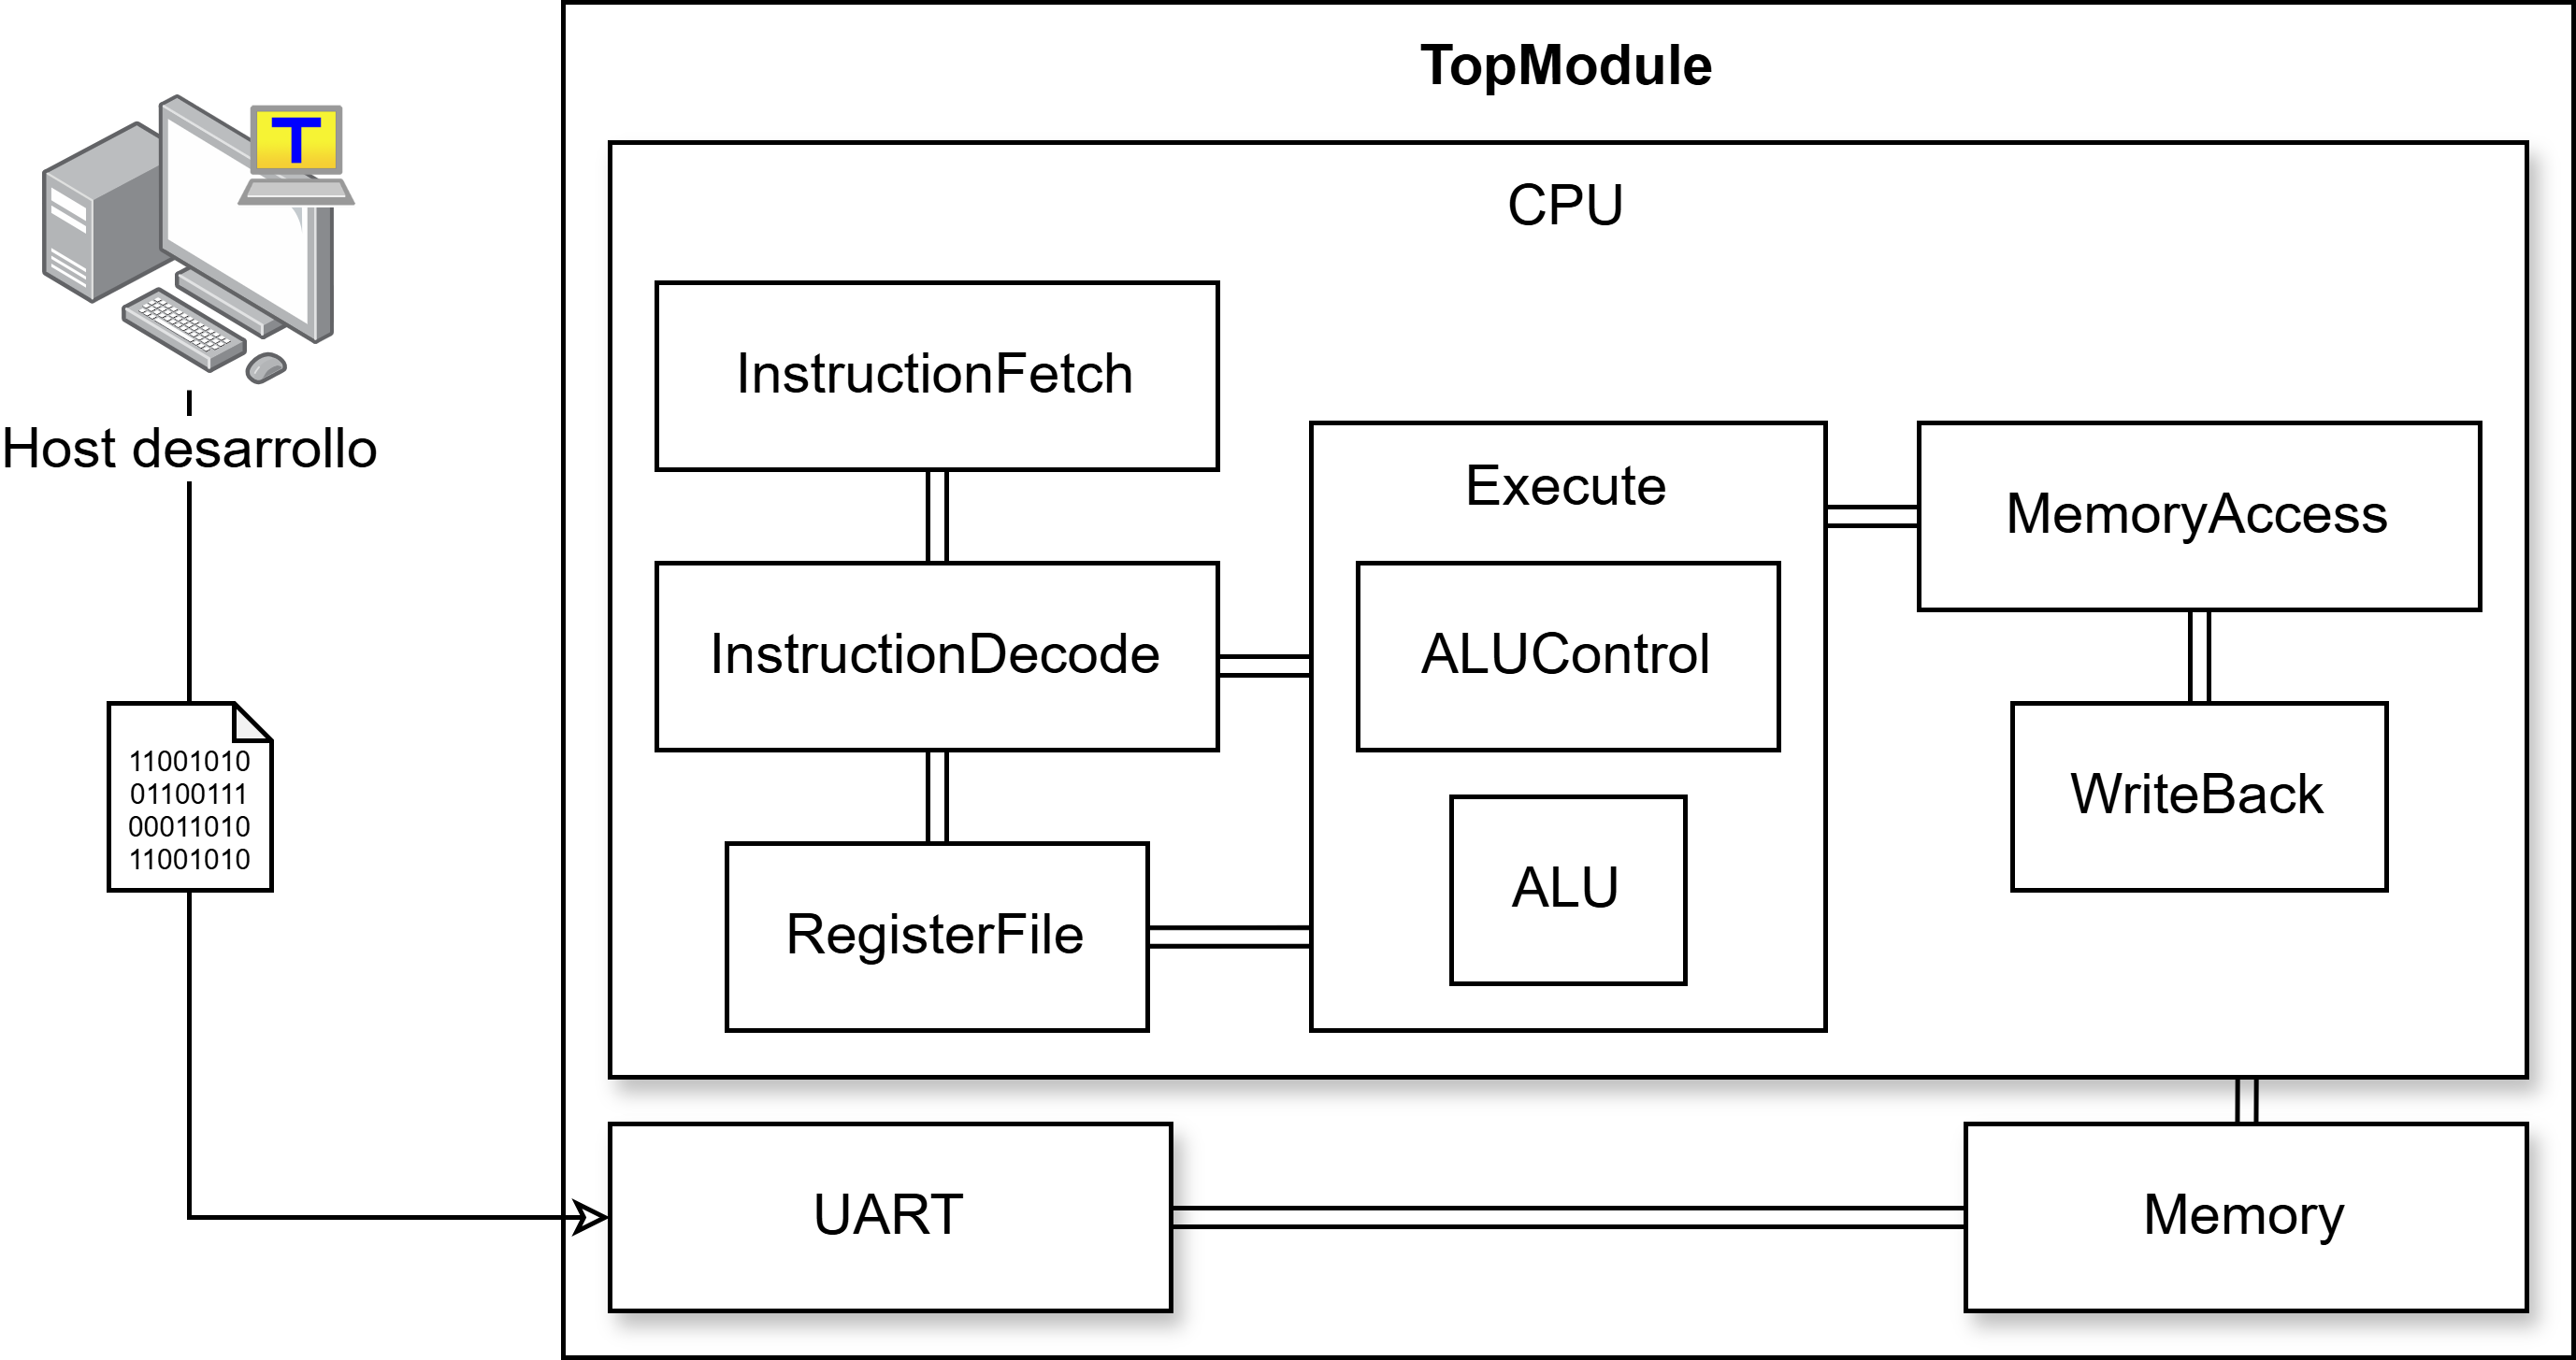
\includegraphics[width=0.7\linewidth]{res/img/diagramas/cap06/01-arquitectura-global-con-uart/arquitectura-global-con-uart.png}
  \caption{Diagrama de bloques con los módulos de los que se compone el computador.}
\end{figure}


%%%%%%%%%%%%%%%%%%%%%%%%%%%%%%%%%%%%%% Proceso de despliegue %%%%%%%%%%%%%%%%%%%%%%%%%%%%%%%%%%%%%%%
\section{Proceso de despliegue}

%%%%%%%%%%%%%%%%%%%%%%%%%%%%%%%%% Obtención del HDL de bajo nivel %%%%%%%%%%%%%%%%%%%%%%%%%%%%%%%%%%
\subsection{Obtención del HDL de bajo nivel}


Por defecto, un fichero de código desarrollado en Chisel no cuenta con un método principal que pueda ejecutarse. Esto es así puesto que la finalidad del código es solamente describir, por medio de constructos propios del lenguaje Scala, el comportamiento interno de componentes hardware. No obstante a esto, el flujo de despliegue de un circuito digital sobre hardware real usando el software Vivado, exige que el punto de entrada de dicho flujo sea código Verilog/VHDL.

Para obtener código Verilog a partir de un desarrollo implementado en Chisel \cite{chisel-to-verilog} es necesario añadir la declaración de objeto mostrada en las líneas 35 a 37 de la Figura 6.2. La instanciación de ese objeto \textit{Top} extendiendo la clase \textit{App} dota al código compilado de un punto de entrada en el que se ejecuta el método \texttt{emitVerilog}, cuyo resultado será una traducción, en sintaxis Verilog, del código Chisel con que se define el módulo \texttt{Top}.

A partir de este fichero Verilog, Vivado llevará a cabo las etapas de síntesis, implementación y generación del \textit{bitstream}\footnote{El bitstream describe cómo debe configurarse el tejido programable de la FPGA, incluyendo la configuración de LUTs, registros, bloques de memoria, redes de interconexión y recursos de entrada/salida.} que posteriormente se programará en el chip FPGA de la placa de desarrollo.

% Figura 6.2: Implementación de la CPU completa, con la definición del punto de entrada a la función que genera el circuito en lenguaje Verilog.
\vspace{+1cm}
\begin{figure}[h!]
\begin{lstlisting}[style=scalaStyle]
class Top extends Module {

  val io = IO(new Bundle {
    val instruction_valid = Input(Bool())
    val i_uart_rx         = Input(Bool())
    val pc_val            = Output(UInt(4.W))
  })
  
  val cpu  = withReset(reset.asAsyncReset) { Module(new CPU) }
  val mem  = Module(new Memory(8192))
  val uart = Module(new UART)

  withReset(~reset.asBool) {
    uart.io.sw_tx     := io.instruction_valid
    uart.io.i_uart_rx := io.i_uart_rx
    
    mem.io.debug_read_address  := 0.U
    cpu.io.instruction_valid   := io.instruction_valid
    mem.io.instruction_address := cpu.io.instruction_address
    cpu.io.instruction         := mem.io.instruction

    cpu.io.debug_read_address  := 7.U
    io.pc_val := cpu.io.instruction_address

    when(!io.instruction_valid) {
      uart.io.mem_bundle <> mem.io.bundle
      cpu.io.memory_bundle.read_data := 0.U
    } .otherwise {
      uart.io.mem_bundle.read_data := 0.U
      cpu.io.memory_bundle <> mem.io.bundle
    }
  }
}

object Top extends App {
  (new chisel3.stage.ChiselStage).emitVerilog(new Top())
}
\end{lstlisting}
\caption{Implementación de la CPU completa, con la definición del punto de entrada a la función que genera el circuito en lenguaje Verilog.}
\end{figure}

\vspace{+0.1cm}
El computador cuenta con las siguientes señales de entrada y salida, las cuales han sido añadidas para trabajar con la FPGA:

\begin{itemize}
  \item \textbf{\textit{instruction\_valid} (entrada)}: La señal con la que se establece si el computador debe permanecer a la espera de recibir el programa o si, por el contrario, debe dar comienzo a su ejecución.
  \vspace{-0.2cm}
  \item \textbf{\textit{i\_uart\_rx} (entrada)}: la entrada de datos del móulo UART.
  \vspace{-0.2cm}
  \item \textbf{\textit{pc\_val} (salida)}: el valor del contador de programa.
\end{itemize}



%%%%%%%%%%%%%%%%%%%%%%%%%%%% Configuración del fichero de constraints %%%%%%%%%%%%%%%%%%%%%%%%%%%%%%
\subsection{Configuración del fichero de \textit{constraints}}

Para asociar la entrada/salida del módulo al hardware disponible en la placa es necesario crear un fichero de \textit{constraints} en el que se indique, por cada puerto de entrada/salida en el módulo, el componente hardware al cual se conectará físicamente.

Se muestran en la Figura 6.3 las asignaciones realizadas para probar el diseño final.

% Figura 6.3: Constraints configurados para probar el multiplexor de dos entradas en la placa.
\vspace{+0.4cm}
\begin{figure}[h!]
\begin{lstlisting}[style=XDCStyle,columns=fullflexible]{}
# Se mapea la señal de control de inicio del programa sobre uno de los interruptores deslizantes
set_property -dict { PACKAGE_PIN A8  IOSTANDARD LVCMOS33 } [get_ports { io_instruction_valid }];

# Se mapea la entrada de datos el módulo UART a la salida del UART de la placa
set_property -dict { PACKAGE_PIN A9  IOSTANDARD LVCMOS33 } [get_ports { io_i_uart_rx }];

# Mapeo de los 4 bits menos significativos del PC sobre 4 diodos LED monócromos
set_property -dict { PACKAGE_PIN H5  IOSTANDARD LVCMOS33 } [get_ports { io_pc_val[0] }];
set_property -dict { PACKAGE_PIN J5  IOSTANDARD LVCMOS33 } [get_ports { io_pc_val[1] }];
set_property -dict { PACKAGE_PIN T9  IOSTANDARD LVCMOS33 } [get_ports { io_pc_val[2] }];
set_property -dict { PACKAGE_PIN T10 IOSTANDARD LVCMOS33 } [get_ports { io_pc_val[3] }];

# Mapeo del del reloj y la señal de reset a los pines correspondientes en la placa
set_property -dict { PACKAGE_PIN E3  IOSTANDARD LVCMOS33 } [get_ports { clock }];
set_property -dict { PACKAGE_PIN C2  IOSTANDARD LVCMOS33 } [get_ports { reset }];

# Definición de la señal de reloj que empleará Vivado en el análisis
create_clock -add -name sys_clk_pin -period 10.00 -waveform {0 5} [get_ports { clock }];
\end{lstlisting}
\vspace{-0.1cm}
\caption{\textit{Constraints} configurados para probar el diseño final en la placa.}
\end{figure}

El reloj de la placa de desarrollo funciona, por defecto, a una frecuencia de 100 MHz. A esa frecuencia de trabajo resulta muy complicado observar las actualizaciones del contador de programa que se reflejan en el array de LEDs, por lo que se ha implementado un divisor de frecuencia con el que ralentizar la ejecución de los programas en la CPU.

El código que implementa el mecanismo se muestra en la Figura 6.4 y su funcionamiento es como sigue:

\subsubsection{Clase \texttt{SlowTick}}
La clase SlowTick alberga un registro empleado como contador incremental. Este contador se incrementa en una unidad a cada ciclo, y se resetea al alcanzar el valor indicado por el parámetro \textit{divisor}. Al resetearse, este módulo genera un pulso de un ciclo de duración en su única salida (valor 1 en el puerto \textit{tick}).

\subsubsection{Clase \texttt{BUFGCE}}
El módulo \texttt{BUFGCE} no define ningún hardware en sí mismo, si no que constituye una referencia a un componente definido fuera del código, bien sea un hardware que no puede ser descrito en Chisel, o un componente físico presente en el hardware donde se vaya a desplegar el diseño. Esto se consigue haciendo que el módulo extienda la clase \texttt{BlackBox}, con lo que se indica, precisamente, que el módulo no se encuentra definido en Chisel.

En este caso, el hardware al que se hace referencia es un buffer de reloj presente en la placa de desarrollo \cite{bufgce-description}. El buffer recibe como entradas una señal de reloj (\texttt{io.I}) y una señal de habilitación (\texttt{io.CE}) de tal modo que, siempre que la señal de habilitación esté activa, se deje pasar a través del buffer un pulso del reloj (puerto de salida \texttt{io.O}).

Lo que proporciona la clase definida en el código es una interfaz para poder interactuar con el buffer y, cuando Vivado reciba el código Verilog del diseño, reconocerá la instanciación del módulo \texttt{BUFGCE} como una primitiva propia de Xilinx, sustituyéndolo por el recurso físico correspondiente.

\subsubsection{Modificaciones en el módulo \texttt{Top}}
En primer lugar, se crean las instancias de los módulos \texttt{SlowTick} y \texttt{BUFGCE} (señales \texttt{slow} y \texttt{gate}, respectivamente). La entrada \texttt{io.I} del \texttt{BUFGCE} será la señal de reloj implícita de Chisel y, la señal de habilitación será el pulso generado por \texttt{SlowTick} cada \texttt{Parameters.ClockMult} ciclos.

Por último, se genera la instancia del módulo \texttt{CPU} indicando que la señal de reloj que gobierne su comportamiento no será la implícita de Chisel, si no la generada por el buffer de reloj.

Si por ejemplo se configurase \texttt{SlowTick} para generar el pulso cada $5 \times 10^{7}$ ciclos, la duración del ciclo observada por el computador sería de:

\[
\underbrace{\frac{1}{100 \cdot 10^{6}}}_{\text{Período del reloj}}
\cdot
\underbrace{5 \cdot 10^{7}}_{\text{Número de ciclos}}
=
0.5\,\text{s}
\]

% Figura 6.4: Implementación de los módulos SlowTick y BUFGCE, y modificaciones realizadas en el módulo Top.
\vspace{+0.2cm}
\begin{figure}[h!!!]
\begin{lstlisting}[style=scalaStyleSmaller]
class SlowTick(divisor: Int) extends Module {
    val io = IO(new Bundle {
      val tick = Output(Bool())
    })
    withReset(~reset.asBool) {
      val counter = RegInit(0.U(32.W))
      counter := Mux(counter === (divisor-1).U, 0.U, counter + 1.U)
      io.tick := (counter === 0.U)
    }
}

class BUFGCE extends BlackBox(Map("CE_TYPE" -> StringParam("\"SYNC\""))) {
  val io = IO(new Bundle {
    val I  = Input(Clock())
    val CE = Input(Bool())
    val O  = Output(Clock())
  })
}

class Top extends Module {
  ...
  val slow = Module(new SlowTick(Parameters.ClockMult))
  val gate = Module(new BUFGCE)
  gate.io.I  := clock
  gate.io.CE := slow.io.tick
  val clk_slow = gate.io.O
  val cpu      = withClockAndReset(clk_slow, reset.asAsyncReset) { Module(new CPU) }
  ...
}
\end{lstlisting}
\vspace{-0.1cm}
\caption{Implementación de los módulos \texttt{SlowTick} y \texttt{BUFGCE}, y modificaciones realizadas en el módulo \texttt{Top}.}
\end{figure}

%%%%%%%%%%%%%%% Análisis de los resultados temporales y de área obtenidos en Vivado %%%%%%%%%%%%%%%%
\section{Análisis de los resultados temporales y de área obtenidos en Vivado}

La integración del \texttt{BUFGCE} tenía el único propósito de hacer que la verificación de resultados de una prueba de concepto (carga y ejecución de un código sencillo), fuera algo realizable, pudiendo observar una actualización del contador de programa cada 0.5 segundos. No obstante, de cara a realizar un análisis de la arquitectura en condiciones normales de operación, se ha suprimido el \texttt{BUFGCE}, quedando en las \textit{constraints}, tan solo, la asignación del reloj al pin correspondiente en la placa, y la definición del reloj \texttt{sys\_clk\_pin}.

A continuación se comentarán los resultados obtenidos por la herramienta Vivado tras la síntesis e implementación del diseño monociclo original y el diseño segmentado.

\subsection{Análisis de la utilización}

En la Figura 6.5 se muestra una tabla en la que se comparan los valores de utilización obtenidos con el comando \texttt{report\_utilization -hierarchical} en la consola \texttt{Tcl} de Vivado. En primer lugar, se observa un decremento del 7\% en el número de LUTs\footnote{\textit{Look-Up Table}: el bloque básico de lógica combinacional de una FPGA. Estos bloques implementan por sí solos cualquier función lógica de un número determinado de entradas.} ocupados por el núcleo (dato de la instancia 'cpu' en la columna 'Logic LUTs').
La incorporación de la \textit{hazard unit} al pipeline, al ser esta una pieza de lógica combinacional tan sencilla, no ha supuesto un incremento en el área del núcleo. No obstante a esto, la memoria ocupa aproximadamente el 80\% de la implementación (en términos de LUTs totales), por lo que, aún siendo algo singular, un decremento del 7\% en el área del núcleo podría entrar dentro de lo esperado. Podría atribuirse, quizás, a las optimizaciones introducidas en el proceso de síntesis.

Un resultado esperado es el incremento del 30\% observado en el número de Flip-Flops (columna 'FF'), como consecuencia directa de la introducción de los registros de segmentación.

% Figura 6.5: Comparativa de los resultados de utilización obtenidos.
\vspace{+0.1cm}
\begin{figure}[H]
\centering
\renewcommand{\arraystretch}{1}
\begin{tabular}{|p{0.95\textwidth}|}
\hline
\textbf{CPU monociclo} \\
\hline
\begin{lstlisting}[style=RiscVStyleSmaller]
     Instance    |      Module  | Total LUTs | Logic LUTs | LUTRAMs | SRLs |  FFs
+----------------+--------------+------------+------------+---------+------+------+
  Top            |        (top) |      11457 |       3265 |    8192 |    0 | 1192
    (Top)        |        (top) |          0 |          0 |       0 |    0 |    0
    cpu          |          CPU |       1906 |       1906 |       0 |    0 | 1146
      inst_fetch |   InstrFetch |       1226 |       1226 |       0 |    0 |  122
      regs       | RegisterFile |        664 |        664 |       0 |    0 | 1024
    mem          |       Memory |       9464 |       1272 |    8192 |    0 |    0
    uart         |         UART |         87 |         87 |       0 |    0 |   46
      uartRx     |   UartRx_mem |         86 |         86 |       0 |    0 |   31
\end{lstlisting}
\\
\hline
\textbf{CPU segmentada} \\
\hline
\begin{lstlisting}[style=RiscVStyleSmaller]
     Instance    |  Module      | Total LUTs | Logic LUTs | LUTRAMs | SRLs |  FFs
+----------------+--------------+------------+------------+---------+------+-----+
  Top            |        (top) |      11200 |       3008 |    8192 |    0 | 1589
    (Top)        |        (top) |          0 |          0 |       0 |    0 |    0
    cpu          |          CPU |       1771 |       1771 |       0 |    0 | 1543
      regs       | RegisterFile |        577 |        577 |       0 |    0 |  992
      srDE       |           DE |        698 |        698 |       0 |    0 |  194
      srEM       |           EM |        381 |        381 |       0 |    0 |  108
      srFD       |      FD__mod |         49 |         49 |       0 |    0 |   98
      srMW       |           MW |         33 |         33 |       0 |    0 |  104
    mem          |       Memory |       9342 |       1150 |    8192 |    0 |    0
    uart         |         UART |         87 |         87 |       0 |    0 |   46
      uartRx     |   UartRx_mem |         85 |         85 |       0 |    0 |   31
\end{lstlisting}
\\
\hline
\end{tabular}
\caption{Comparativa de los resultados de utilización obtenidos.}
\end{figure}

\subsection{Análisis temporal}

En el resumen del análisis temporal obtenido con el comando \texttt{report\_timing\_summary} se indican los siguientes valores para el WNS (\textit{Worst Negative Slack}) de cada diseño:

\begin{itemize}
  \item \textbf{Monociclo:} WNS (ns) = -19.983
  \item \textbf{Segmentado:} WNS (ns) = 0.058
\end{itemize}

El WNS es un valor que representa el margen temporal más desfavorable del diseño. En otras palabras, es la diferencia entre el tiempo de ciclo marcado como objetivo de la implementación (en este caso, 10 ns), y el tiempo que corresponde al camino crítico. Un valor negativo del WNS indica que existe al menos una ruta que no cumple con el tiempo de ciclo especificado.

A partir de las cifras obtenidas puede inferirse que la frecuencia máxima a la que puede trabajar el computador monociclo es de

\[
F_{\text{max}}=
\frac{1}{T_{\text{crit}}}
=
\frac{1}{T_{\text{reloj}}-WNS}
=
\frac{1}{10-(-19.983)}
=
33.35 MHz
\]

donde $T_{\text{crit}}$ es el tiempo que tarda una señal en recorrer el camino crítico, y $T_{\text{reloj}}$ es el periodo de la señal de reloj ($1/f_{\text{reloj}}$). Por otro lado, al haber obtenido un slack positivo para el diseño segmentado, este podrá funcionar a los 100 MHz que marca el reloj de la placa.

Al ejecutar el comando \texttt{report\_timing -max\_paths 5} se obtiene un informe más detallado con los datos presentado en la Figura 6.6. Se observa el slack obtenido para cada implementación, el requisito temporal a cumplir (periodo del reloj en el apartado \textit{Requirement}), el tiempo del camino crítico (dato del apartado \textit{Data Path Delay}), y el número de niveles lógicos atravesados en ese camino crítico (\textit{Logic Levels}).

% Figura 6.6: Selección de algunos de los valores obtenidos tras análisis temporal.
\vspace{+0.1cm}
\begin{figure}[H]
\centering
\renewcommand{\arraystretch}{1}
\begin{tabular}{|p{0.95\textwidth}|}
\hline
\textbf{CPU monociclo} \\
\hline
\begin{lstlisting}[style=RiscVStyleSmaller]
Slack (VIOLATED) :    -19.983ns  (required time - arrival time)
  Requirement:        10.000ns  (sys_clk_pin rise@10.000ns - sys_clk_pin rise@0.000ns)
  Data Path Delay:    29.924ns  (logic 4.604ns (15.386%)  route 25.320ns (84.614%))
  Logic Levels:       24  (LUT2=1 LUT3=1 LUT5=2 LUT6=13 MUXF7=4 MUXF8=1 RAMD64E=2)
\end{lstlisting}
\\
\hline
\textbf{CPU segmentada} \\
\hline
\begin{lstlisting}[style=RiscVStyleSmaller]
Slack (MET) :         0.058ns  (required time - arrival time)
  Path Group:         sys_clk_pin
  Path Type:          Setup (Max at Slow Process Corner)
  Requirement:        10.000ns  (sys_clk_pin rise@10.000ns - sys_clk_pin rise@0.000ns)
  Data Path Delay:    9.583ns  (logic 2.231ns (23.282%)  route 7.352ns (76.718%))
  Logic Levels:       11  (CARRY4=4 LUT3=1 LUT4=1 LUT6=5)
\end{lstlisting}
\\
\hline
\end{tabular}
\caption{Selección de algunos de los valores obtenidos tras análisis temporal.}
\end{figure}

En resumen, gracias a la segmentación se ha conseguido reducir el tiempo del camino crítico en, aproximadamente, 20 ns, lo cual se traduce en una frecuencia de trabajo 3 veces superior o, lo que es lo mismo, se ha logrado un speedup de x3, alejado del x5 ideal, pero igualmente significativo.